\chapter{Wazuh Übersicht}
\section{Entstehung}
Wazuh ist aus dem Open-Source Projekt \href{https://github.com/ossec}{ossec}\footnote{Link: https://github.com/ossec} entstanden.
Wazuh ist wie ossec komplett Open-Source und kostenlos verfügbar.

\section{Aufbau}
Wazuh basiert auf dem \acrfull{elk} Stack und besteht aus einem Manager und den Agents. 
Der Manager ist ein Plugin, welches in den \acrshort{elk} Stack integriert werden kann und mithilfe von Agents auf den Computern Logdateien sammelt.

\begin{figure}[H]
    \centering
    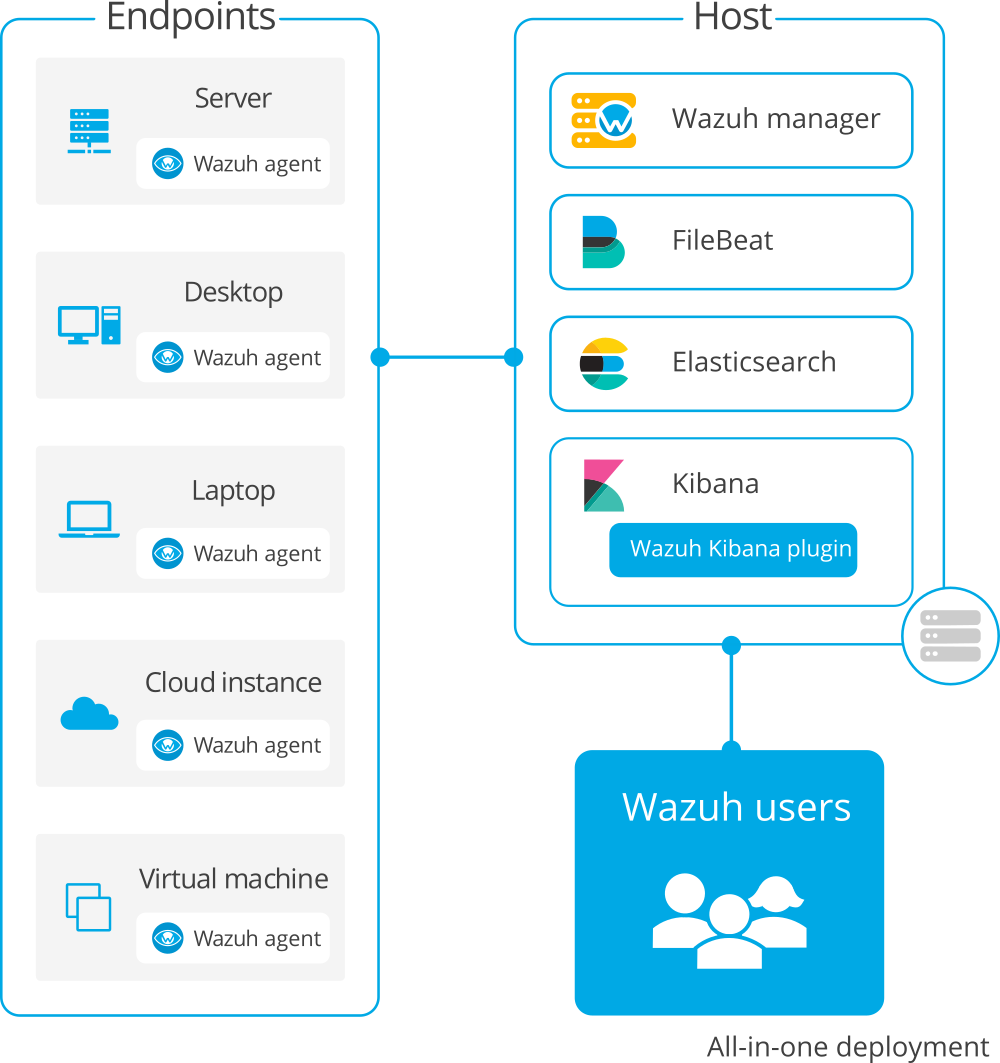
\includegraphics[width=0.5\linewidth]{../img/aufbau-wazuh.png}
    \caption[Übersicht Wazuh]{Übersicht Wazuh\footnotemark}
\end{figure}
\footnotetext{Zugriff: 24.04.2022 \cite{wazuh-documentation}}


\section{Prozessablauf}
Die Agents senden die Logeinträge an den Wazuh Manager.
Danach werden die Logeinträge mit einem Decoder strukturiert und die Regeln werden auf die Logeinträge angewendet.
Wenn eine Regel zutrifft, wird ein Alert generiert und angezeigt.
Wenn keine Regel zutrifft, wird der Logeintrag verworfen.
In der ossec.conf kann eingestellt werden, dass auch die Logeinträge abgespeichert werden, die auf keine Regel zutreffen.
Dabei sammeln sich grosse Datenmengen an und dies ist hauptsächlich für Debugging empfohlen.

\begin{figure}[H]
    \centering
    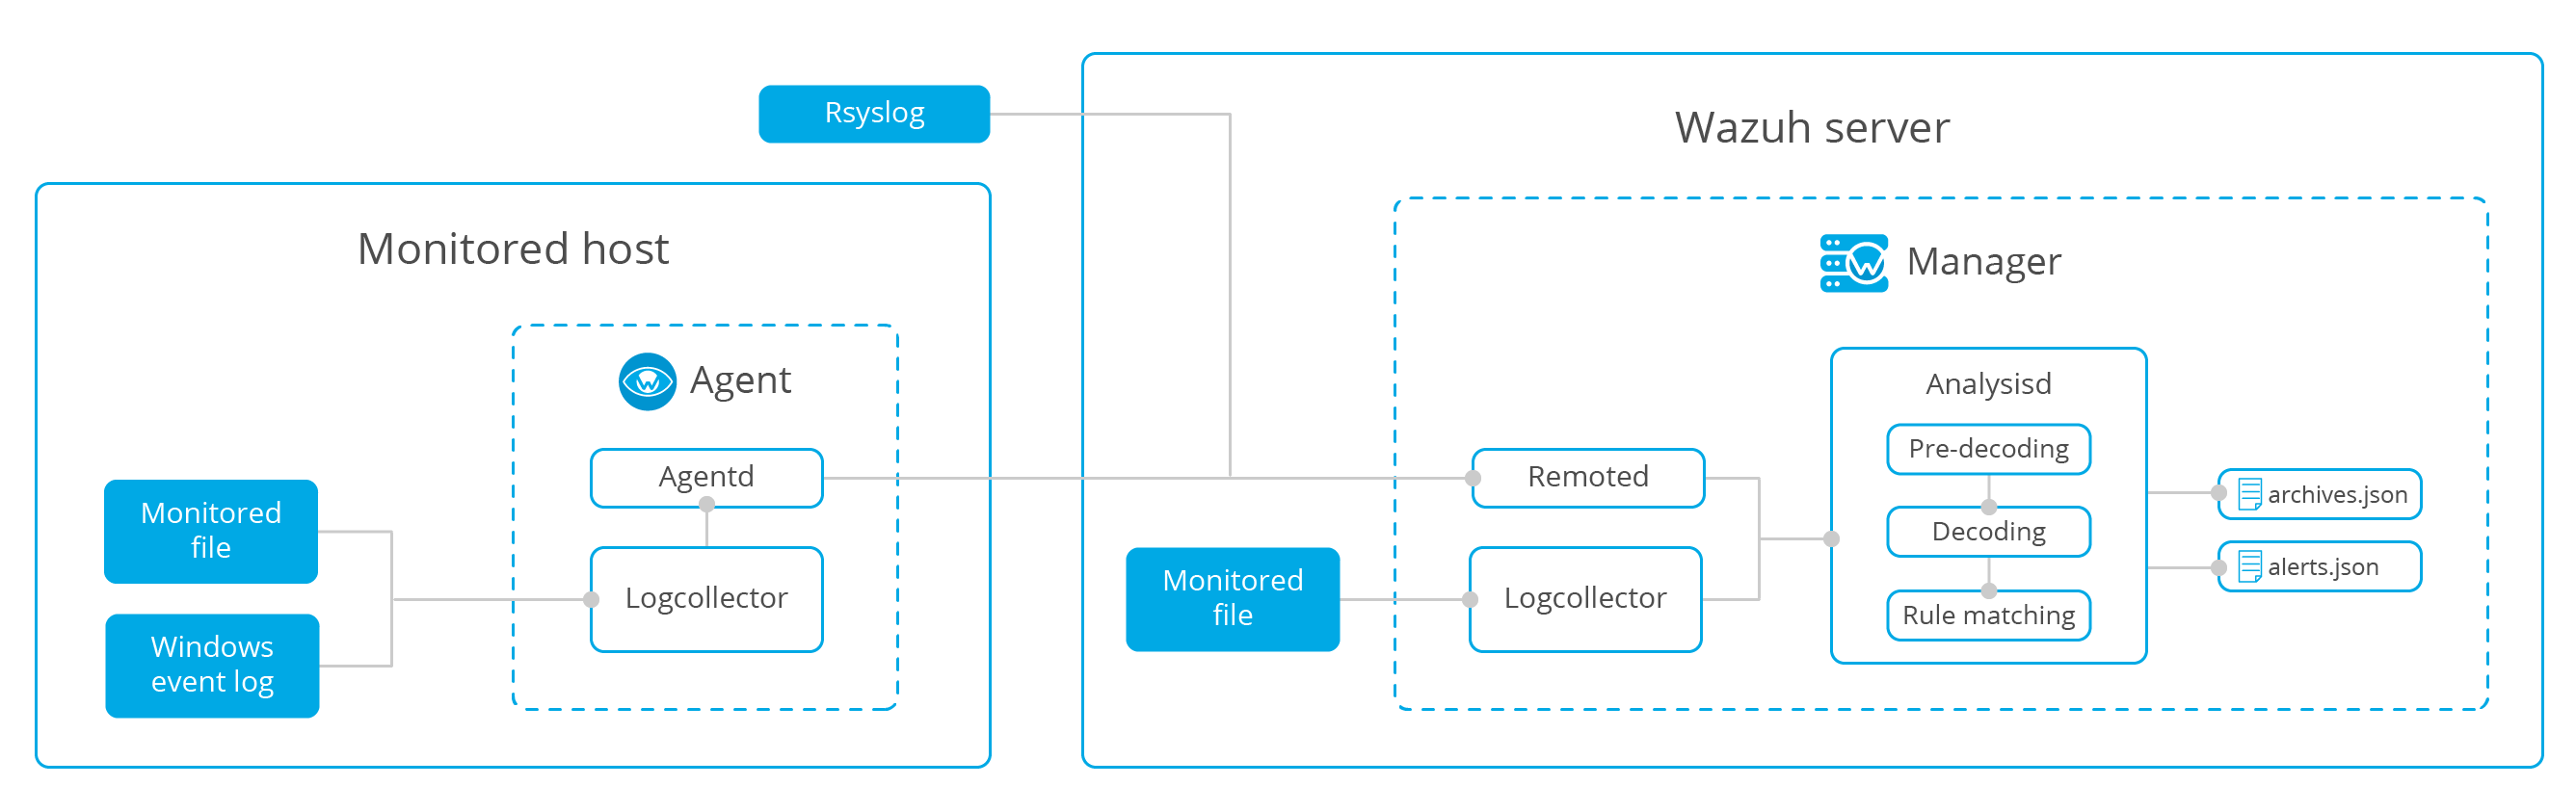
\includegraphics[width=\linewidth]{../img/wazuh-ablauf.png}
    \caption[Wazuh Ablauf]{Wazuh Ablauf\footnotemark}
\end{figure}
\footnotetext{Zugriff: 24.04.2022 \cite{wazuh-documentation}}


\section{Wazuh Manager}
Der Wazuh Manager wird auf einem Linux Server installiert und beinhaltet den kompletten \acrshort{elk} Stack, mit Wazuh Plugin. 
Er ist verantwortlich für die Verarbeitung der eingehenden Logeinträge. 
Dazu werden Groups, Decoder und Rules verwendet. 

\subsection{Groups}
Die Gruppen werden verwendet, um ähnliche Geräte zu gruppieren.
Für jede Gruppe kann man eine agent.conf einrichten, in welcher eingetragen wird welche Logdateien von diesen Systemen verarbeitet werden sollen. 

\subsubsection{agent.conf}
In der agent.conf kann definiert werden, welche Logdateien an den Wazuh Manager weitergeleitet werden. 
Eine Lokation wird mit <localfile> angegeben:
\begin{lstlisting}
<agent_config os="Windows">
    <localfile>
        <location>Microsoft-Windows-Sysmon/Operational</location>
        <log_format>eventchannel</log_format>
    </localfile>
</agent_config>
\end{lstlisting}
Weitere Informationen wie neue Orte mit Logdateien eingebunden werden können, findet man in der \href{https://documentation.wazuh.com/current/user-manual/reference/centralized-configuration.html?highlight=agent%20conf}{Wazuh Dokumentation}\footnote{Link: https://documentation.wazuh.com/current/user-manual/reference/centralized-configuration.html?highlight=agent\%20conf}\\

\subsection{Decoders}
Da Logs in allen möglichen Formen daherkommen, je nach Herkunft braucht es verschiedene Decoder.
Die Decoder bringen die eingehenden Logs in eine einheitliche Struktur, um die Regeln darauf anwenden zu können.
Es werden Decoder für einige bekannten Logformate angeboten, wie zum Beispiel für den Windows Event Manager oder Cisco IOS Logs.\\



\subsection{Rules}


\subsubsection{Alert Level}
Es gibt Alert Levels von 0 bis 16. 
Diese bedeuten nicht wie schwerwiegend ein Ereignis ist, sondern jedes Level hat eine spezielle Bedeutung.
Die wichtigsten Level sind folgende:
\begin{itemize}
    \item \textbf{Level 3} sind Alerts, welche authorisiert sind und tendenziell nicht gefährlich.
    \item \textbf{Level 12} sind Alerts, welche eine Anomalie darstellen und potenziell gefährlich sind.
\end{itemize}

Alle Alert Level findet man in der \href{https://documentation.wazuh.com/current/user-manual/ruleset/rules-classification.html}{Wazuh Dokumentation}\footnote{Link: https://documentation.wazuh.com/current/user-manual/ruleset/rules-classification.html}.


\subsection{Konfiguration}
In der ossec.conf Datei sind alle Konfigurationen vom Wazuh-Manager abgespeichert.
Die Konfigurationsdatei kann im \acrshort{gui} bearbeitet werden. Alternativ liegt die Datei unter:
\begin{lstlisting}
    /var/ossec/etc/ossec.conf
\end{lstlisting}


\section{Wazuh Agent}
Der Wazuh Agent wird auf dem Client installiert.
Es werden die meisten Betriebssysteme unterstützt. Darunter viele Linux Systeme, Windows und MacOS.\\

Der Wazuh Agent leitet alle Logdateien, die in der agent.conf definiert sind, weiter an den Wazuh Manager.
Zusätzlich überwacht der Wazuh Agent auch alle Systemdatei- und Registryänderungen und leitet diese an den Wazuh Manager weiter. 
